\chapter{Material layup for optimized designs: KB1 to KB4}
\label{ch:material_layup_KB1_KB4}
%-------------------------------------------------------------
% KB1
%------------------------------------------------------------
\section{Material layup for KB1}

Figures \ref{fig:KB1matstackr01} to \ref{fig:KB1matstackr07} show the material stacking and thicknesses in the KB1 blade. 

\begin{figure}[pth]
\begin{center}
	\includegraphics[width=.85\linewidth]{figures/KB1_region01.eps}
\end{center}
\caption{Material thicknesses in the trailing edge reinforcement of the KB1 blade.}
\label{fig:KB1matstackr01}
\end{figure}

\begin{figure}[pth]
\begin{center}
	\includegraphics[width=.85\linewidth]{figures/KB1_region02.eps}
\end{center}
\caption{Material thicknesses in the main panel (immediately behind the spar cap) of the KB1 blade.}
\label{fig:KB1matstackr02}
\end{figure}

\begin{figure}[pth]
\begin{center}
	\includegraphics[width=.85\linewidth]{figures/KB1_region04.eps}
\end{center}
\caption{Material thicknesses in the spar cap of the KB1 blade.}
\label{fig:KB1matstackr04}
\end{figure}

\begin{figure}[pth]
\begin{center}
	\includegraphics[width=.85\linewidth]{figures/KB1_region06.eps}
\end{center}
\caption{Material thicknesses in the leading region (immediately in front of the spar cap) of the KB1 blade.}
\label{fig:KB1matstackr06}
\end{figure}

\begin{figure}[pth]
\begin{center}
	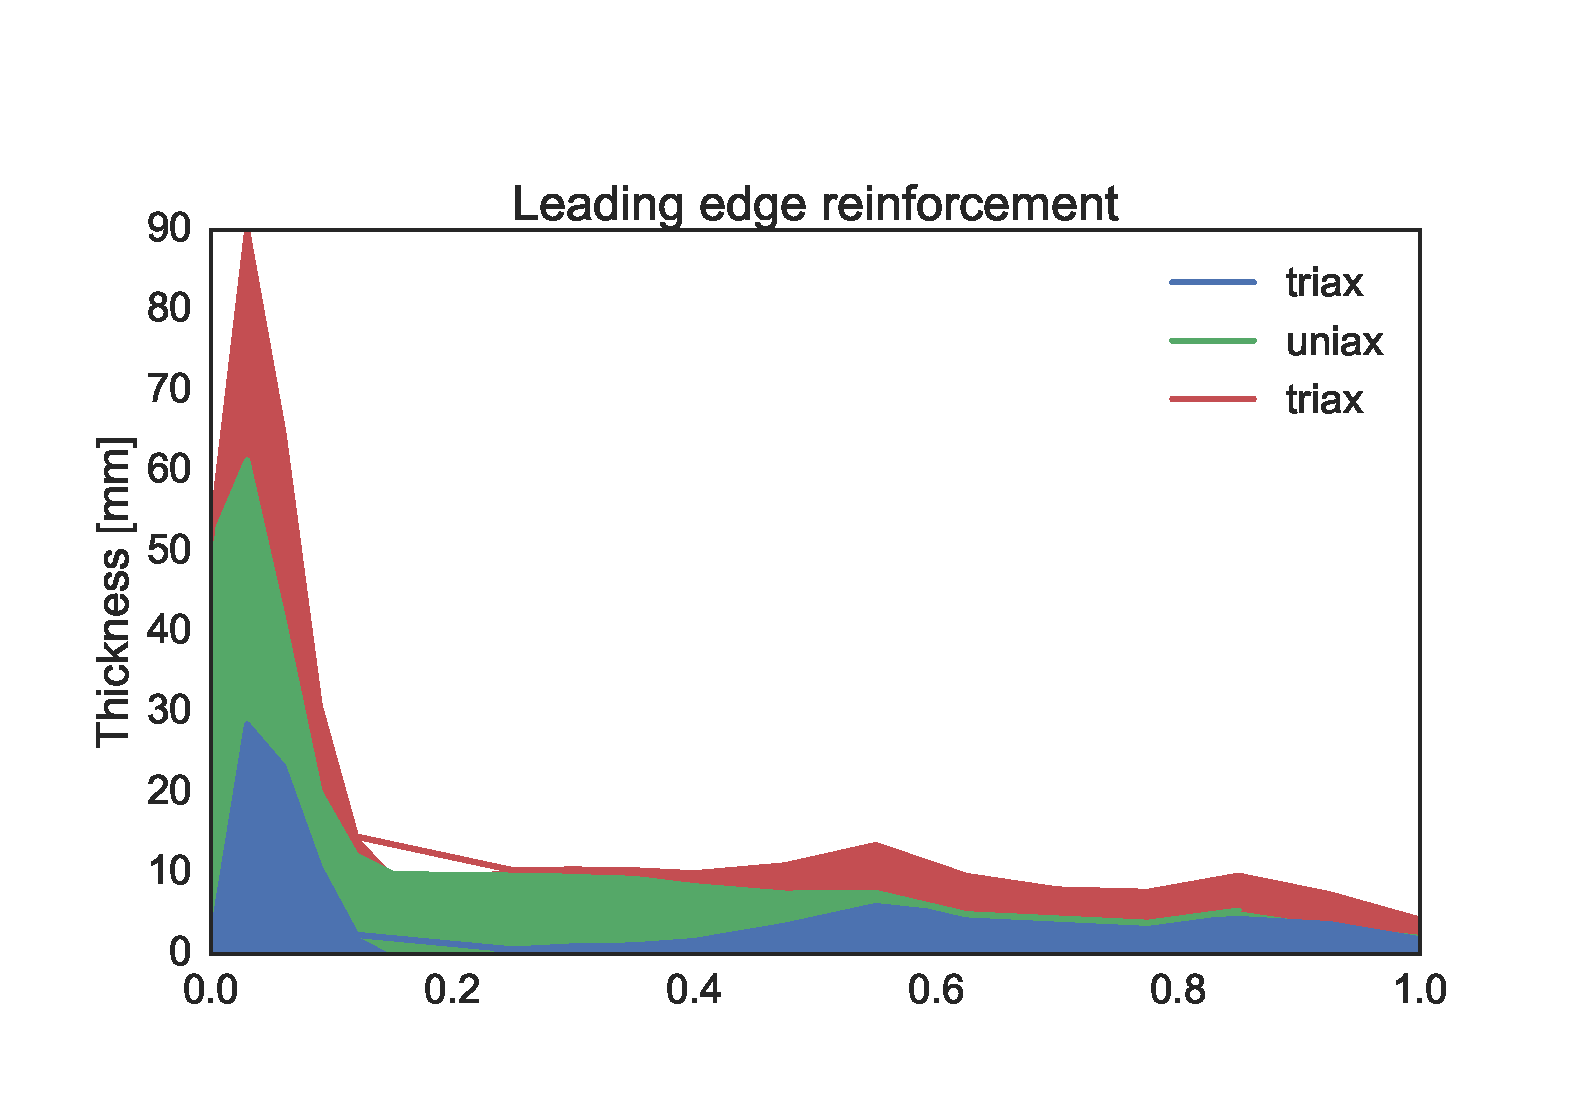
\includegraphics[width=.85\linewidth]{figures/KB1_region07.eps}
\end{center}
\caption{Material thicknesses in the leading edge reinforcement of the KB1 blade.}
\label{fig:KB1matstackr07}
\end{figure}

%-------------------------------------------------------------
% KB2
%------------------------------------------------------------
\section{Material layup for KB2}
Figures \ref{fig:KB2matstackr01} to \ref{fig:KB2matstackr07} show the laminate layup in the KB2 blade.

\begin{figure}[pth]
\begin{center}
	\includegraphics[width=.85\linewidth]{figures/KB2_region01.eps}
\end{center}
\caption{Material thicknesses in the trailing edge reinforcement of the KB2 blade.}
\label{fig:KB2matstackr01}
\end{figure}

\begin{figure}[pth]
\begin{center}
	\includegraphics[width=.85\linewidth]{figures/KB2_region02.eps}
\end{center}
\caption{Material thicknesses in the main panel (immediately behind the spar cap) of the KB2 blade.}
\label{fig:KB2matstackr02}
\end{figure}

\begin{figure}[pth]
\begin{center}
	\includegraphics[width=.85\linewidth]{figures/KB2_region04.eps}
\end{center}
\caption{Material thicknesses in the spar cap of the KB2 blade.}
\label{fig:KB2matstackr04}
\end{figure}

\begin{figure}[pth]
\begin{center}
	\includegraphics[width=.85\linewidth]{figures/KB2_region06.eps}
\end{center}
\caption{Material thicknesses in the leading region (immediately in front of the spar cap) of the KB2 blade.}
\label{fig:KB2matstackr06}
\end{figure}

\begin{figure}[pth]
\begin{center}
	\includegraphics[width=.85\linewidth]{figures/KB2_region07.eps}
\end{center}
\caption{Material thicknesses in the leading edge reinforcement of the KB2 blade.}
\label{fig:KB2matstackr07}
\end{figure}
%-------------------------------------------------------------
% KB3
%------------------------------------------------------------
\section{Material layup for KB3}
Figures \ref{fig:KB3matstackr01} to \ref{fig:KB3matstackr07} show the material layup in the KB3 optimized blade.

\begin{figure}[pth]
\begin{center}
	\includegraphics[width=.85\linewidth]{figures/KB3_region01.eps}
\end{center}
\caption{Material thicknesses in the trailing edge reinforcement of the KB3 blade.}
\label{fig:KB3matstackr01}
\end{figure}

\begin{figure}[pth]
\begin{center}
	\includegraphics[width=.85\linewidth]{figures/KB3_region02.eps}
\end{center}
\caption{Material thicknesses in the main panel (immediately behind the spar cap) of the KB3 blade.}
\label{fig:KB3matstackr02}
\end{figure}

\begin{figure}[pth]
\begin{center}
	\includegraphics[width=.85\linewidth]{figures/KB3_region04.eps}
\end{center}
\caption{Material thicknesses in the spar cap of the KB3 blade.}
\label{fig:KB3matstackr04}
\end{figure}

\begin{figure}[pth]
\begin{center}
	\includegraphics[width=.85\linewidth]{figures/KB3_region06.eps}
\end{center}
\caption{Material thicknesses in the leading region (immediately in front of the spar cap) of the KB3 blade.}
\label{fig:KB3matstackr06}
\end{figure}

\begin{figure}[pth]
\begin{center}
	\includegraphics[width=.85\linewidth]{figures/KB3_region07.eps}
\end{center}
\caption{Material thicknesses in the leading edge reinforcement of the KB3 blade.}
\label{fig:KB3matstackr07}
\end{figure}
%-------------------------------------------------------------
% KB4
%------------------------------------------------------------
\section{Material layup for KB4}
Figures \ref{fig:KB4matstackr01} to \ref{fig:KB4matstackr07} show the laminate layup in the KB4 blade.

\begin{figure}[pth]
\begin{center}
	\includegraphics[width=.85\linewidth]{figures/KB4_laminate_layers_r01.eps}
\end{center}
\caption{Material thicknesses in the trailing edge reinforcement of the KB4 blade.}
\label{fig:KB4matstackr01}
\end{figure}

\begin{figure}[pth]
\begin{center}
	\includegraphics[width=.85\linewidth]{figures/KB4_laminate_layers_r02.eps}
\end{center}
\caption{Material thicknesses in the main panel (immediately behind the spar cap) of the KB4 blade.}
\label{fig:KB4matstackr02}
\end{figure}

\begin{figure}[pth]
\begin{center}
	\includegraphics[width=.85\linewidth]{figures/KB4_laminate_layers_r04.eps}
\end{center}
\caption{Material thicknesses in the spar cap of the KB4 blade.}
\label{fig:KB4matstackr04}
\end{figure}

\begin{figure}[pth]
\begin{center}
	\includegraphics[width=.85\linewidth]{figures/KB4_laminate_layers_r06.eps}
\end{center}
\caption{Material thicknesses in the leading region (immediately in front of the spar cap) of the KB4 blade.}
\label{fig:KB4matstackr06}
\end{figure}

\begin{figure}[pth]
\begin{center}
	\includegraphics[width=.85\linewidth]{figures/KB4_laminate_layers_r07.eps}
\end{center}
\caption{Material thicknesses in the leading edge reinforcement of the KB4 blade.}
\label{fig:KB4matstackr07}
\end{figure}
